%%
%% This is file `./samples/longsample.tex',
%% generated with the docstrip utility.
%%
%% The original source files were:
%%
%% apa7.dtx  (with options: `longsample')
%% ----------------------------------------------------------------------
%% 
%% apa7 - A LaTeX class for formatting documents in compliance with the
%% American Psychological Association's Publication Manual, 7th edition
%% 
%% Copyright (C) 2019 by Daniel A. Weiss <daniel.weiss.led at gmail.com>
%% 
%% This work may be distributed and/or modified under the
%% conditions of the LaTeX Project Public License (LPPL), either
%% version 1.3c of this license or (at your option) any later
%% version.  The latest version of this license is in the file:
%% 
%% http://www.latex-project.org/lppl.txt
%% 
%% Users may freely modify these files without permission, as long as the
%% copyright line and this statement are maintained intact.
%% 
%% This work is not endorsed by, affiliated with, or probably even known
%% by, the American Psychological Association.
%% 
%% ----------------------------------------------------------------------
%% 
\documentclass[man,floatsintext]{apa7}
\usepackage[american]{babel}
\usepackage{csquotes}
\usepackage[style=apa,sortcites=true,sorting=nyt,backend=biber]{biblatex}
\usepackage{amsmath, amssymb, geometry, graphicx, booktabs}
\DeclareLanguageMapping{american}{american-apa}
\addbibresource{normalized-rank-comparison.bib}

\title{A \textsf{Novel} Method for Ranking Group Performance}
\shorttitle{Normalized Rank Dominance}

\author{Kartikeya Mishra}
\authorsaffiliations{Independent Researcher}

\leftheader{Mishra}

\abstract{
This paper introduces a novel non-parametric method for calculating group-level performance scores, incorporating rank sums, weight bias adjustments for unequal group sizes, and cross-collection interpretability. Theoretical derivations, Empirical validations and detailed example are discussed.
}

\keywords{Normalized Rank Comparison, Performance Analysis, Weighted Bias Adjustment, Group Performance Metrics, Statistical Methods}

\authornote{
   \addORCIDlink{Kartikeya Mishra}{0009-0001-3311-3955}
   %add the link when research paper is complete and fill the details in the orcid to add the link

  Correspondence concerning this article should be addressed to Kartikeya Mishra 50-D, Block E-3, Shatabdi Vihar, Sector 52, Noida, UP - 201307, India. E-mail: kartik.maxwell@gmail.com}

\begin{document}
\maketitle
This formula can numerically identify the performance of a group $P_i$ within a collection of groups containing uneven number of elements. This novel approach takes into account weight bias inherent in the formula itself. The performance value, $P_i$ numerically falls in the normalized range of [0,1] from non-dominant to dominant performance within their collection, which gives a more interpretable and practical scale, which could be visualized as 0 to 100\% dominance in performance via $P_i * 100$. 
This standardized scale can be used to compare within cross-collection which have different scales, see the \hyperref[fig:superset-collection]{Figure 1} to which , this formula can be applied towards.
\begin{figure}[!htb]
    \caption{Superset Collection of Elementary Grade Groups and High School Groups}
    \centering
    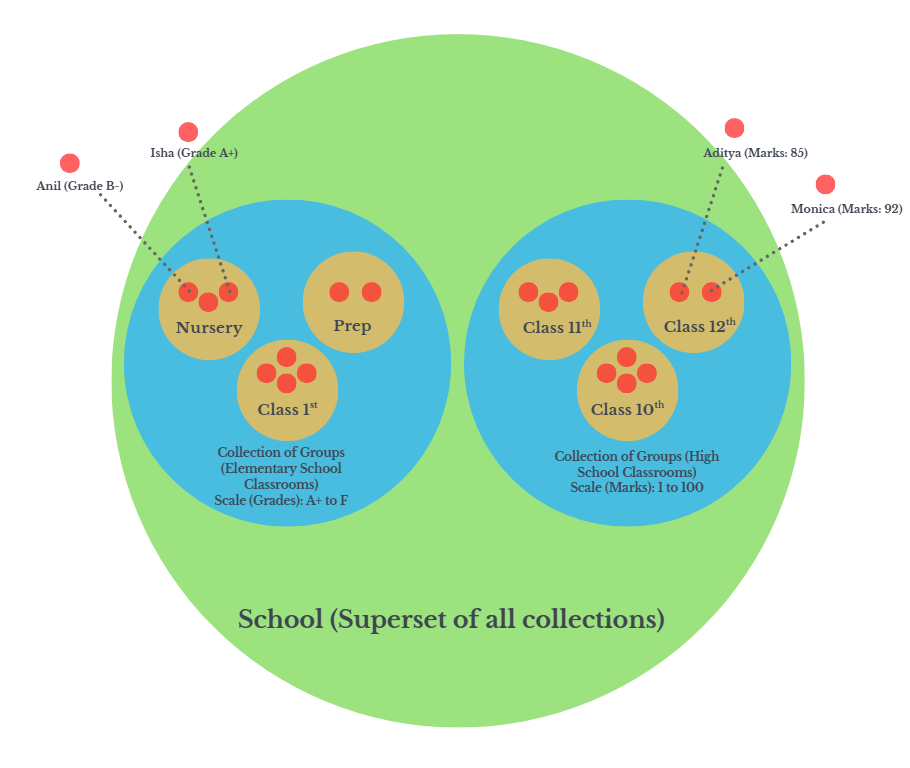
\includegraphics [scale=0.5]{images/superset_collection.png}
    \label{fig:superset-collection}
\end{figure}

The inspiration for the formula came from the idea from \cite{mann1947test}, which uses median to calculate p-value significance. Though, the idea is inspired from their, but applied in terms of assessing performance comparison
for groups having uneven elements, and expanded to create a standardize scale with cross-collection interpretability.

\section{Normalized Group Performance Assessment Formulae}


\begin{equation}
\boxed{
\mathbf{
P_i = \frac{-n_i +  \sum\limits_{j=1}^{n_i} r_j}{n_i \cdot (N - 1)}}
}
\end{equation}
   
\begin{itemize}
    \item \textbf{Ranks}: Sequential ranks assigned to items within and across groups. Tied ranks are averaged out. Note ranks are in ascending order of dominance i.e. rank 1 is the lowest, with rank $N^{th}$ as the highest. This is done to keep symmetry with usage of ranks in other statistics methods such as \cite{mann1947test} etc.
    \item \textbf{$P_i$}: Normalized Performance value in the range of [0, 1]
    \item \textbf{$\sum r_i$}: Sum of ranks for group $i$.
    \item \textbf{$n_i$}: number of elements within the $i^{th}$ group
    \item \textbf{$N$}: Total number of elements across all group combined. \hfill \break
    There are \[k = \text{number of groups}, \quad n_i = \text{number of items in each group }\]
    \begin{align}
        \text{N} = \sum\limits_i^k n_i, \quad \text{where N = total number of items}
    \end{align}

\end{itemize}

\subsection{Applications}
This is a list of Applications scenario, the formula was designed for:
\begin{itemize}
    \item \textbf{Educational}: Awarding Best Class Performance in a school, when classes have uneven students, and even different grading scales.
    \item \textbf{Organizational}: To identify best-performing team in the organization, and least-performing, for restructuring and guidance purposes, when number of person per team are uneven, and performance scale at various sector of an organization is different.
   \item \textbf{Business}: Often businesses have economy segment and luxury segment for services and products. Often, just price is not an enough indicator what segment of products fared better. If, a ranking is created, on customer feedback, return on investment, less-after-cost-maintenance, expenses etc. Then, this formula can be used to find the dominant product/services of their business, when there is uneven sale of each product/services sold.
\end{itemize}
There could be applications outside the scope of this paper. But, when designing the formula these above listed applications were being thought of.

\hfill \break
Mathematical derivation, along with its theoretical justification, would be discussed, with its analogous visual intuition where possible. Maxima and Minima, range of dominance [0, 1], would be proven as well.

\section{Non-normalized Performance}

If you see, the \hyperref[fig:dominance_Understanding]{Figure 2}, is intuitively easy to understand that Group B performance is more dominant, that Group A, simply because Group B occupy the higher ranks, and Group A lower ranks.
\begin{figure}[!htb]
    \caption{Visual intuition of the Dominance Formula, where Dominance: Group B > Group A}
    \centering
    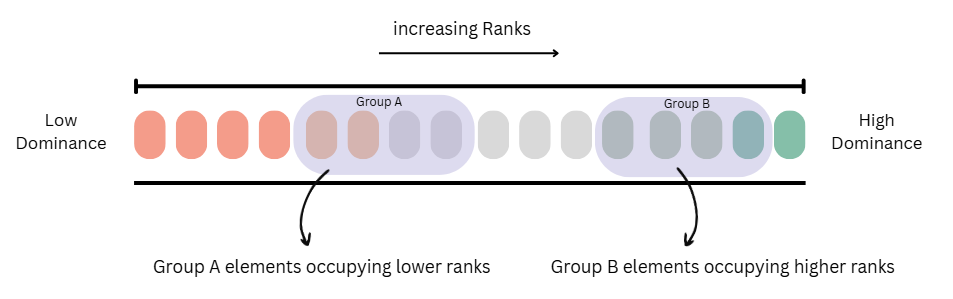
\includegraphics[scale=0.65]{images/dominance-intuition.png}
    \label{fig:dominance_Understanding}
\end{figure}

This non-normalized performance value, with uneven number of groups is given by:
\begin{equation}
\label{eq:non-normalized}
    p_i^{(non-normalized)} = w_i \cdot \frac{\sum r_i}{ S_{UDH} }
\end{equation}
This later non-normalized dominance would be used to derive the normalized version of the formula. Therefore, non-normalized performance derivation would be discussed first.

\begin{itemize}
    \item Sum of Upper Dominant Half ($S_{UDH}$):
    \begin{align}
        S_{UDH} = \frac{N(N+1)}{2} - \frac{a(a+1)}{2}, \quad a = \lfloor N/2 \rfloor
    \end{align}
    \item Weight Bias ($w_i$):
    \begin{align}
        w_i = \frac{N}{k n_i}
    \end{align}
\end{itemize}

\subsection*{Derivation of Non-normalized Performance}
From, the understanding we gain from \hyperref[fig:dominance_Understanding]{Figure 2}, we can easily, ascertain the local dominance, if we divide the scale into two halves of lower ranks half, and upper rank half. So, the group with ranks in the upper half would have a more prominent or dominant performance. So, we need to figure out what's the ranks of the upper dominant half is.

\subsubsection{Sum of Upper Dominant Half}
\begin{enumerate}
\item{Purpose of UDH}
The \textbf{Upper Dominant Half (UDH)} represents the \textbf{rank sum of the dominant half} of a dataset, providing a benchmark for performance potential in rank-based comparisons.

\item{Total Rank Sum (Full Dataset)}
For a dataset with \textbf{N items}, the \textbf{total rank sum} is the sum of integers from \textbf{1 to N}:
\begin{equation}
S = 1 + 2 + 3 + \ldots + N
\end{equation}
Using the formula for the sum of the first \( N \) integers:
\begin{equation}
S = \frac{N(N + 1)}{2}
\end{equation}

\item{Split the Dataset into Halves}
\begin{itemize}
  \item \( a = \lfloor \frac{N}{2} \rfloor \) represents the size of the \textbf{non-dominant half} (lower half).
  \item The \textbf{dominant upper half} includes the rank from \( a + 1 \) to \(N^{th}\) rank items.
\end{itemize}



\item{Rank Sum of Non-Dominant Half (Lower Half)}
The \textbf{non-dominant half} (lower half) consists of the \textbf{smallest \( a \) ranks}. Its rank sum is:
\begin{equation}
S_{lower} = 1 + 2 + \ldots + a
\end{equation}
Using the formula for sum of integers:
\begin{equation}
S_{lower} = \frac{a(a+1)}{2}
\end{equation}

\item{Rank Sum of Dominant Half (Upper Half)}
The \textbf{Upper Dominant Half} is calculated by subtracting the rank sum of the \textbf{lower half} from the \textbf{total rank sum}:
\begin{equation}
S_{UDH} = S - S_{lower}
\end{equation}
Substituting the formulas:
\begin{equation}
S_{UDH} = \frac{N(N + 1)}{2} - \frac{a(a+1)}{2}
\end{equation}

\item{Final Formula}
\begin{equation}
\label{eq:SUDH}
S_{UDH} = \frac{N(N + 1)}{2} - \frac{a(a+1)}{2}
\end{equation}

\begin{itemize}
  \item \( N \): Total number of items.
  \item \( a \): Size of the lower \textbf{dominant half}, calculated as the floor of half of the net total number of items across all groups, so as to be inclusive of both odd and even count of N items:
  \begin{equation}
  a = \lfloor \frac{N}{2} \rfloor
  \end{equation}
\end{itemize}
\end{enumerate}

\subsubsection*{Non-normalized Performance Formulae (Biased)}
So, to if we compare the ranked sum of the group with the upper dominant half, we can get a numerical understanding of performance value
\begin{equation}
\label{eq:p-biased}
    p_i^{(biased)} = \frac{\sum r_i}{ S_{UDH} }
\end{equation}
\begin{itemize}
    \item \textbf{$\sum r_i$}: Sum of ranks for group $i$.
    \item \textbf{$S_{UDH}$}: Sum of Upper Dominant Half
\end{itemize}

As, the formula doesn't take into account weight bias. A high number of items can still occupy lower ranks, but in account of total items in group being large, its ranked sum also gives a higher value. That's why weigh bias was added to adjust this non-normalized performance value.

\subsubsection*{Weight Bias Derivation}
To derive the weight bias ($w_i$), we first understand, that if all the groups have equal number of items, then $w_i = 1$ i.e. no adjustment needed. That means all the groups have the same number of elements in them. The items expected in each group, can be written as:
\begin{equation}
X_e = \frac{N}{k}
\end{equation}
where:
\begin{itemize}
    \item $X_e$: Expected item count per group.
    \item $k$: Number of groups in collection.
    \item $N$: Total number of items across all groups.
\end{itemize}

So, now we calculate the fractional change needed to reach expected group item
\begin{equation}
 fractional \ change = \frac{X_e - n_i}{n_i}
\end{equation}

If we want to adjust our biased performance, $p_i^{(biased)}$, according to the fractional change, 
then,
\begin{equation}
    p_i^{(unbiased)} = p_i^{(biased)} +  p_i^{(biased)} *  fractional \ change
\end{equation}

in other words, taking $p_i^{(biased)}$ as common, we can rewrite it as
\begin{equation}
\label{eq:p-unbiased}
    p_i^{(unbiased)} = p_i^{(biased)} * (1 +  fractional \ change)
\end{equation}

So, the term needed to adjust from $p_i^{(biased)}$ to $p_i^{(unbiased)}$, can be written as:
\begin{equation}
    w_i = 1 + fractional \ change
\end{equation}

substituting everything we get, the derivation of weight bias:
\begin{equation}\label{eq:weight-bias}
    w_i = \frac{N}{kn_i}
\end{equation}

where:
\begin{itemize}
    \item $w_i$: Weight bias for group $i$.
    \item $n_i$: Number of items in group $i$.
    \item $N$: Total number of items.
    \item $k$: Number of groups.
\end{itemize}

\subsubsection{Final Formula for unbiased (but non-normalized) Performance Value}
Therefore, from \hyperref[eq:SUDH]{Equation 12}, \hyperref[eq:p-biased]{Equation 14},  \hyperref[eq:p-unbiased]{Equation 18}, and \hyperref[eq:weight-bias]{Equation 20}

we derived unbiased(but non-normalized) formulae, as stated in the beginning of the section, in \hyperref[eq:non-normalized]{Equation 3}:
\begin{equation}
    p_i^{(non-normalized)} = w_i \cdot \frac{\sum r_i}{ S_{UDH} }
\end{equation}

Note in this research paper, $p_i^{(non-normalized)}$ = $p_i^{(unbiased)}$ are same, but for standardization sake, we will use $p_i^{(non-normalized)}$ moving forward.


\subsection{Theoretical Justification}

We explicitly derive this adjustment to satisfy several criteria:
\begin{itemize}
    \item The adjustment explicitly becomes smaller as the number of groups $k$ or total observations $N$ increases, ensuring minimal interference in larger datasets.
    Mathematically, we justify the chosen form by observing its desirable properties in handling various scenarios:

\begin{align*}
\lim_{N \to \infty} \frac{8}{k(3N+2)} &= 0, \\
\lim_{k \to \infty} \frac{8}{k(3N+2)} &= 0.
\end{align*}
    \item Explicitly provides a meaningful zero baseline for dominance measures.
    \item dominance scores become standardized, allowing direct comparisons across multiple studies or scenario
\end{itemize}




\subsection*{Derivation of Adjustment Term}

We aim to minimize the dominance measure $U_i^{(local)}$ defined as:
\begin{equation}
U_i^{(local)} = w_i \cdot \frac{\sum r_i}{S_{UDH}}
\end{equation}

This is locally valid dominance measure for a single collection.

Now, if we always assume that the net total number of items across all groups is even, it is safe to assume explicitly that:

\begin{equation}
a = \frac{N}{2}
\end{equation}

Thus, the lower and upper halves would be explicitly:
\[
\left[1, \frac{N}{2}\right] \quad \text{and} \quad \left[\frac{N}{2}+1, N\right]
\]

Simplifying explicitly, we get:

\begin{align*}
S_{UDH} &= \frac{N}{2} \times \frac{\left(\frac{N}{2} + 1 + N\right)}{2} \\
&= \frac{N}{4} \times \frac{3N + 2}{2} \\
&= \frac{N(3N + 2)}{8}
\end{align*}

Now explicitly substituting everything into our dominance equation:

\begin{align*}
U_i &= \frac{N}{k n_i} \times \frac{\sum r_i \times 8}{N(3N + 2)} \\
&= \frac{8}{k n_i} \times \frac{\sum r_i}{3N + 2}
\end{align*}

This explicitly represents the simplified and explicitly minimized form of the dominance measure.




\subsection*{Minimizing Expression}

For the given expression to be minimized, $\sum r_i$ should be low. Consider exdplicitly:

\begin{equation}
\frac{\sum r_i}{n_i} = \frac{\frac{n_i}{2}(1+n_i)}{n_i} = \frac{1}{2}(n_i + n_i^2)
\end{equation}

Differentiating explicitly and setting to zero for minimization:

\begin{equation}
\frac{d}{d n_i}\left[\frac{1}{2}(n_i + n_i^2)\right] = \frac{1}{2}(1 + 2 n_i) = 0
\end{equation}

Solving explicitly, we find:

\begin{equation}
n_i = -\frac{1}{2}
\end{equation}

Explicitly confirming via second derivative:

\begin{equation}
\frac{d^2}{d n_i^2}\left[\frac{1}{2}(n_i + n_i^2)\right] = 1
\end{equation}

The second derivative explicitly indicates a minimum. However, explicitly, since $n_i$ represents a countable quantity and cannot be negative or fractional, we evaluate explicitly at the nearest valid positive integer, i.e., $n_i = 1$:

\begin{equation}
f(1) = \frac{1}{2}(1 + 1^2) = 1
\end{equation}

Thus explicitly, the minimum feasible value of the expression $\frac{\sum r_i}{n_i}$ is: 1

\subsection*{Minimum Dominance Value Analysis}

This explicitly indicates that the lowest dominance value occurs when there is a singular group within the collection having one element with the lowest rank. Additionally, explicitly, the number of groups ($k$) and total number of items ($N$) across all groups should be high.

Therefore, explicitly, the minimum dominance value depends on the term:

\begin{equation}
\frac{8}{k(3N+2)}
\end{equation}

\subsection{Final Adjusted Dominance Score}

The dominance score, explicitly adjusted, is presented as:
\begin{equation}
\mathbf{
U_i = U_i^{(local)} - \frac{8}{k(3N+2)}
}
\end{equation}

Thus explicitly, the adjusted dominance measure is both fairer and more interpretable across diverse datasets.

\section{Validation of Dominance Formula}
\begin{itemize}
    \item Mathematical proof of sympy
    \item Numerical proof annd implementation in Python 
    \item cross-validation from a different method
\end{itemize}

\section{Detailed Example of Dominance Method}

To explicitly demonstrate the utility and robustness of the normalized dominance scoring method, we consider a complex example meeting the following conditions:
\begin{itemize}
    \item Multiple groups (in example four groups)
    \item Unequal number of items per group (minimum three items per group)
    \item Tied ranks
    \item Odd total number of participants ($N=15$)
\end{itemize}

\subsection{Data and Initial Rankings}

Participants from four intervention groups (A, B, C, D) were ranked based on their effectiveness scores. Ties were assigned average ranks explicitly in \hyperref[initial-data]{Table 1}:

\begin{table}[htbp!]
\centering
\caption{Effectiveness Scores and Verified Assigned Ranks}
\begin{tabular}{llcc}
\toprule
Participant & Group & Score & Rank \\
\midrule
1 & A & 95 & 13.5 (tie) \\
2 & A & 48 & 9 \\
3 & A & 25 & 6 \\
4 & A & 15 & 2.5 (tie) \\
5 & B & 83 & 12 \\
6 & B & 57 & 10 \\
7 & B & 100 & 15 \\
8 & C & 70 & 11 \\
9 & C & 20 & 5 \\
10 & C & 40 & 8 \\
11 & D & 95 & 13.5 (tie) \\
12 & D & 15 & 2.5 (tie) \\
13 & D & 18 & 4 \\
14 & D & 30 & 7 \\
15 & D & 10 & 1 \\
\bottomrule
\end{tabular}
\label{initial-data}
\end{table}

\subsection{Calculations}

\textbf{Step 1: Rank Sums}
\begin{itemize}
\item $r_A = 13.5 + 9 + 6 + 2.5 = 31$
\item $r_B = 12 + 10 + 15 = 37$
\item $r_C = 11 + 5 + 8 = 24$
\item $r_D = 13.5 + 2.5 + 4 + 7 + 1 = 28$
\end{itemize}

\textbf{Step 2: Define Parameters}

Total participants: $N=15$, Number of groups: $k=4$.

Group sizes:
\begin{itemize}
\item $n_A = 4$, $n_B = 3$, $n_C = 3$, $n_D = 5$
\end{itemize}

Compute explicitly $a = \lfloor N/2 \rfloor = \lfloor 15/2 \rfloor = 7$.

\textbf{Step 3: Calculate Upper Dominant Half}

Lower Dominant Half (LDH):
\begin{equation}
S_{lower} = \frac{a(a+1)}{2} = \frac{7 \times 8}{2} = 28
\end{equation}

Total sum of ranks:
\begin{equation}
S = \frac{N(N+1)}{2} = \frac{15 \times 16}{2} = 120
\end{equation}

Upper Dominant Half (UDH):
\begin{equation}
S_{UDH} = S - S_{lower} = 120 - 28 = 92
\end{equation}

\textbf{Step 4: Weight Bias Calculation}
\begin{equation}
w_i = \frac{N}{k \cdot n_i}
\end{equation}

Calculate explicitly:
\begin{itemize}
\item $w_A = \frac{15}{4 \times 4} = 0.9375$
\item $w_B = \frac{15}{4 \times 3} = 1.25$
\item $w_C = \frac{15}{4 \times 3} = 1.25$
\item $w_D = \frac{15}{4 \times 5} = 0.75$
\end{itemize}

\textbf{Step 5: Dominance Scores}

Dominance scores explicitly computed as:
\begin{equation}
U_i = w_i \cdot \frac{r_i}{S_{UDH}}
\end{equation}

Calculate:
\begin{itemize}
\item $U_A = 0.9375 \times \frac{31}{92} = 0.316$
\item $U_B = 1.25 \times \frac{37}{92} = 0.503$
\item $U_C = 1.25 \times \frac{24}{92} = 0.326$
\item $U_D = 0.75 \times \frac{28}{92} = 0.228$
\end{itemize}

\subsection{Summary of Dominance Results}
Results have been summarized in \hyperref[dominance-result]{Table 2}
\begin{table}[htb!]
\centering
\caption{Dominance Calculation Results}
\begin{tabular}{lccc}
\toprule
Group & Rank Sum ($r_i$) & Weight Bias ($w_i$) & Dominance Score ($U_i$) \\
\midrule
A & 31 & 0.9375 & 0.316 \\
B & 37 & 1.2500 & 0.503 (Most Dominant) \\
C & 24 & 1.2500 & 0.326 \\
D & 28 & 0.7500 & 0.228 (Least Dominant) \\
\bottomrule
\end{tabular}
\label{dominance-result}
\end{table}

\subsection{Interpretation of Results}

Group B achieves the highest dominance score, demonstrating superior effectiveness. Despite the variations in group size and tied ranks, the method accurately balances these complexities. Group D has the lowest dominance score, emphasizing the method’s robustness and fairness in clearly assessing relative performance.

\subsection{Validation of Results}

\printbibliography
\appendix
\end{document}

%% 
%% Copyright (C) 2019 by Daniel A. Weiss <daniel.weiss.led at gmail.com>
%% 
%% This work may be distributed and/or modified under the
%% conditions of the LaTeX Project Public License (LPPL), either
%% version 1.3c of this license or (at your option) any later
%% version.  The latest version of this license is in the file:
%% 
%% http://www.latex-project.org/lppl.txt
%% 
%% Users may freely modify these files without permission, as long as the
%% copyright line and this statement are maintained intact.
%% 
%% This work is not endorsed by, affiliated with, or probably even known
%% by, the American Psychological Association.
%% 
%% This work is "maintained" (as per LPPL maintenance status) by
%% Daniel A. Weiss.
%% 
%% This work consists of the file  apa7.dtx
%% and the derived files           apa7.ins,
%%                                 apa7.cls,
%%                                 apa7.pdf,
%%                                 README,
%%                                 APA7american.txt,
%%                                 APA7british.txt,
%%                                 APA7dutch.txt,
%%                                 APA7english.txt,
%%                                 APA7german.txt,
%%                                 APA7ngerman.txt,
%%                                 APA7greek.txt,
%%                                 APA7czech.txt,
%%                                 APA7turkish.txt,
%%                                 APA7endfloat.cfg,
%%                                 Figure1.pdf,
%%                                 shortsample.tex,
%%                                 longsample.tex, and
%%                                 bibliography.bib.
%% 
%%
%% End of file `./samples/longsample.tex'.
